\tikzstyle{end} = [thin, circle, minimum size = 0.1cm, draw, inner sep = 0.1pt]
\tikzstyle{leaf} = [thin, circle, minimum size = 0.6cm, draw, inner sep = 0.1pt, blue]
\tikzstyle{inner} = [thin, circle, minimum size = 0.2cm, draw, inner sep = 0.1pt, black]
            


\tikzstyle{ed} = [thick, ->, draw, black]

    
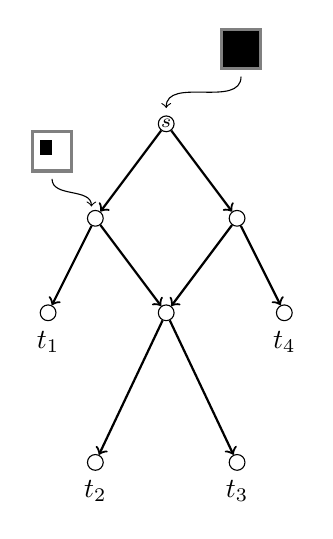
\begin{tikzpicture}
    \node[inner] (a) at (0, 0) {\scriptsize $s$};
    \node[inner] (b) at (-0.9, -1.2) {};
    \node[inner] (c) at (0.9, -1.2) {};
    \node[inner, label = below:$t_1$] (d) at (-1.5, -2.4) {};
    \node[inner] (e) at (0, -2.4) {};
    \node[inner, label = below:$t_4$] (f) at (1.5, -2.4) {};
    \node[inner, label = below:$t_2$] (g) at (-0.9, -4.3) {};
    \node[inner, label = below:$t_3$] (h) at (0.9, -4.3) {};
    
    \path (a) edge[ed] (b);
    \path (a) edge[ed] (c);
    \path (b) edge[ed] (d);
    \path (b) edge[ed] (e);
    \path (c) edge[ed] (e);
    \path (c) edge[ed] (f);
    \path (e) edge[ed] (g);
    \path (e) edge[ed] (h);
    
    \draw[very thick, gray, fill = black] (0.7, 1.2) rectangle (1.2, 0.7);
    \draw[->] (0.95, 0.6) to[out = 270, in = 90] (0, 0.2);

    \draw[very thick, gray] (-1.7, -0.1) rectangle (-1.2, -0.6);
    \fill[black] (-1.6, -0.2) rectangle (-1.45, -0.4);
    \draw[->] (-1.45, -0.7) to[out = 270, in = 90] (-0.95, -1.05);
\end{tikzpicture}
